% Implementation

\section{Principles}
\subsection{The influence of bypassing to SHIP++}
The SHCT stores the history of re-reference intervals for cache blocks, indexed by a signature derived from the block's address. When a cache block is accessed, SHIP++ computes its signature using an improved signature generation mechanism, designed to better capture the access pattern information. The signature is then used to index the corresponding SHCT entry. SHIP++ employs an adaptive update policy for the SHCT entries, allowing it to adjust the prediction mechanism dynamically based on the observed access patterns and cache behavior. Using the updated SHCT entry, SHIP++ predicts the re-reference interval for the accessed cache block, which represents the number of accesses between two consecutive accesses of the same block. The re-reference interval prediction is used to assign a Recency Position (RP) value to the cache block. Cache blocks with higher RP values are considered less likely to be accessed in the near future and are prioritized for eviction\cite{Wu2011}. Due to this, we plan to utilize the SHCT property and combine it with bypass topology to enhance cache performance.\par
Initially, a rudimentary test was conducted, wherein bypassing was implemented when the SHCT value was equated to 0. As depicted in fig.\ref{fig.Picture4}, the performance of this approach is suboptimal, particularly in the case of specific benchmarks such as 434. Upon analysis, it was discovered that this issue also occurred in Homework 2. In Homework 2, bypassing was implemented when the counter value, utilized to track the number of hits, exceeded a specified threshold. Subsequently, an examination of the bypass policy was conducted to gain further insights.\par
\begin{figure*}[htbp]
\centering
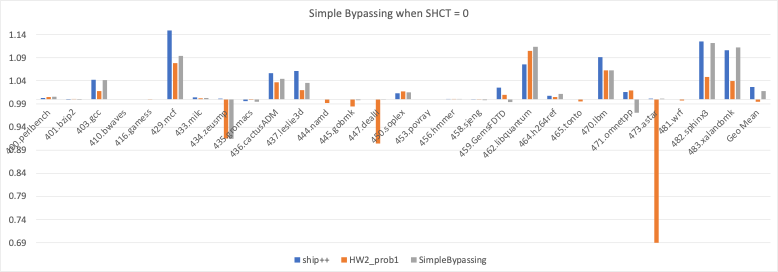
\includegraphics[width=0.9\textwidth]{figs/Picture4.png}
\caption{Simple bypassing when SHCT=0}
\label{fig.Picture4}
\end{figure*}
Bypassing cache replacement can perform well and provide performance improvements in certain situations. When the working set of an application is significantly larger than the cache size, bypassing can help reduce cache pollution by avoiding the storage of blocks that are unlikely to be reused in the near future.  In cases where access patterns are irregular or non-sequential, bypassing can prevent the eviction of frequently accessed cache blocks by avoiding the replacement of blocks with a low likelihood of being accessed again soon. Bypassing can alleviate cache thrashing situations, where cache blocks are continuously evicted and replaced due to the working set size exceeding the cache capacity. By identifying and bypassing blocks with a low reusability potential, cache thrashing can be mitigated, improving overall system performance. If the current cache replacement policy is not achieving a satisfactory cache hit rate, bypassing can help improve cache performance by selectively bypassing blocks that are deemed less likely to be accessed in the near future. In scenarios where data is accessed in a streaming or one-time manner (e.g., multimedia processing or large dataset scans), bypassing cache replacement can prevent the unnecessary eviction of other potentially reusable blocks, ultimately improving cache hit rate and overall performance\cite{Gao2010}. \par
Consequently, in the context of this project, the bypassing strategy is considered ineffective when the majority of reuse distances exceed the number of cache ways present in a set (16). Although the SHCT can determine which signature's reuse distance is below 16, it cannot pinpoint the signature exhibiting the minimum reuse distance when the distance exceeds 16, leading to constant misses. Furthermore, when a signature is marked for bypassing, it is less likely to be accessed in the immediate future, resulting in a prolonged bypassing period. Simultaneously, it is crucial to ensure that bypassed data does not remain within sample sets to avoid hindering future access to such data.\par
Assuming a scenario with only four ways and an access pattern such as A B C D E A F G H I A..., combined with the condition that a block is marked for bypassing after two misses, as observed with the "A" pattern in the example, despite "A" possessing the smallest reuse distance, it might still be bypassed and consequently never accessed in the future. It becomes evident that the performance would be unsatisfactory.\par
To address the issue of cache thrashing, an additional parameter is introduced to count valuable data, such as enumerating the instances of "less than 2" in the Re-Reference Production Value (RRPV). Upon the counter value exceeding a pre-established threshold, determined to be 14 after conducting numerous experiments, bypassing will be implemented. Furthermore, a verification process will be employed to determine if the data is within the sample set. If the data is present in the sample set, it will adhere to the SHIP++ policy; if not, bypassing will be executed.\par 
The results are illustrated in fig. \ref{fig.Picture5}. As demonstrated by this figure, the performance of our policy significantly surpasses that of SHIP++ for benchmarks such as 462. Additionally, improvements are observed for the previously underperforming 434 benchmark.\par 

\begin{figure*}[htbp]
\centering
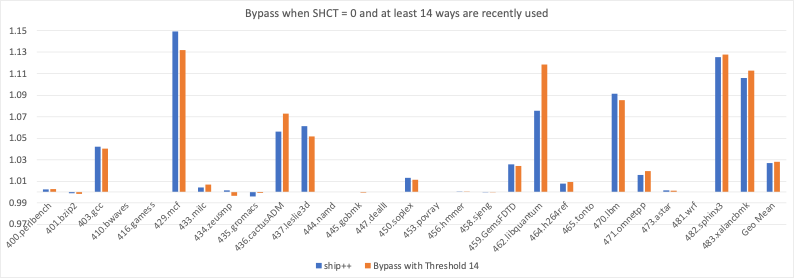
\includegraphics[width=0.9\textwidth]{figs/Picture5.png}
\caption{Bypassing when SHCT=0 and at least 14 ways are recently used}
\label{fig.Picture5}
\end{figure*}

\subsection{The utilization of SHCT}
When the initial value of the SHCT is set to 1, it is noted that the maximum value of the SHCT consistently stays at 1, even after 100 million accesses. This pattern is also persistently observed when the initial values are assigned as 2 and 5. Consequently, this suggests that a considerable portion of the SHCT table remains unutilized, leading to inefficiency and the squandering of resources.
\begin{figure}[htbp]
\centering
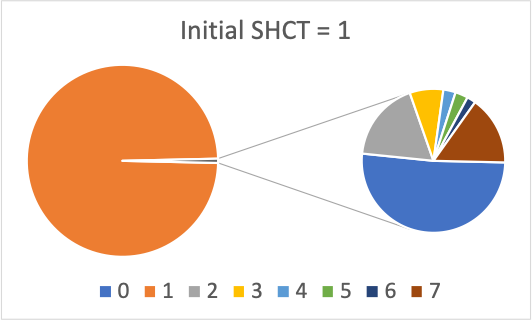
\includegraphics[width=0.4\textwidth]{figs/Picture1.png}
\caption{Initial SHCT = 1}
\label{fig.Picture1}
\end{figure}

\begin{figure}[htbp]
\centering
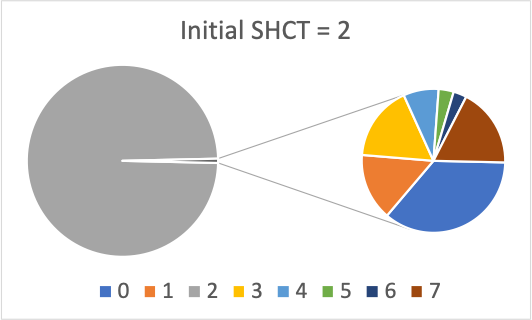
\includegraphics[width=0.4\textwidth]{figs/Picture2.png}
\caption{Initial SHCT = 2}
\label{fig.Picture2}
\end{figure}

\begin{figure}[htbp]
\centering
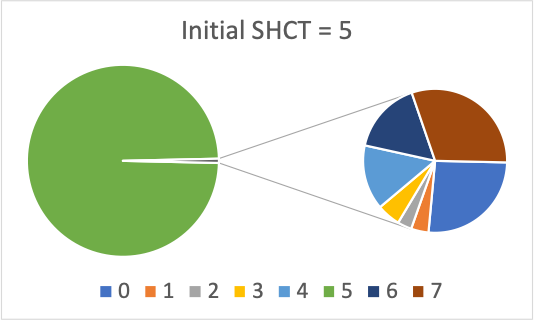
\includegraphics[width=0.4\textwidth]{figs/Picture3.png}
\caption{Initial SHCT = 5}
\label{fig.Picture3}
\end{figure}

SHCT has 16K entries, with each entry consisting of 3 bits. Subsequently, three minor experiments are conducted to further investigate the system.
\begin{itemize}
    \item \(Test 1\): try the smaller size entries like 4K entries,  and keep the same 3 bits.
    \item \(Test 2\): keep the same size entries, try the smaller number bits like 2 bits.
    \item \(Test 3\): try the smaller size entries like 4K entries, and also smaller number bits like 2 bits.
\end{itemize}
The result is illustrated in the fig. \ref{fig.Figure6}. From this depiction, it is evident that the geometric mean across the various configurations is quite similar. Consequently, it is possible to reduce the size of the SHCT table, thereby decreasing the hardware storage requirements.
\begin{figure*}[htbp]
\centering
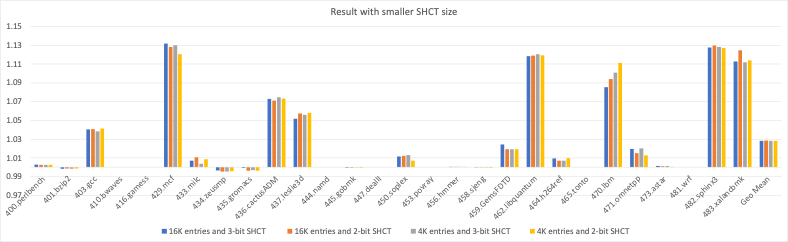
\includegraphics[width=0.9\textwidth]{figs/Picture6.png}
\caption{Result with smaller size}
\label{fig.Figure6}
\end{figure*}